\subsection{Clamped System}
This following section focuses on data extraction and analysis for a system of a clamped graphene sheet with a free standing hexagon membrane in the middle of the sheet. See \cref{}. The free standing hexagon will therefore be a simplified model compared to that of a more realistic model containing two graphene sheets: a constrained sheet with hexagonal holes and a free standing sheet on top. This model will be discussed later. 
\subsubsection{Frequency vs. membrane size}
In order to find the correlation between frequency of the modes in the membrane and the membrane size, the frequency over each membrane, which varies in size, is extracted and plotted as a function of the size of the given membrane. \\
This is done by defining a sheet of a definite size in VNL and thereafter check the frequencies for the different membranes by inserting the different size membranes, one after the other. The distance from the edge of the membrane, to the edge of the sheet (or the next membrane) is called "neck" and has been chosen to be 5 nm for the biggest membrane which has a 10 nm diameter. With this "neck" size it is certain that the membrane do not transfer any energy to each other, according to reports \ref{p} \\
Furthermore, only the frequencies for the first couple of modes will be checked.
\onecolumngrid

\begin{figure}[H]
    \centering
    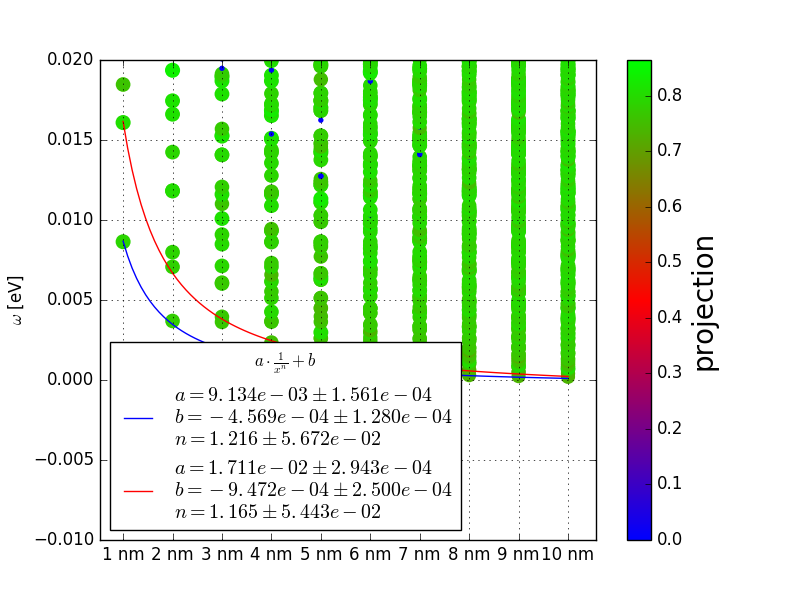
\includegraphics[width=\columnwidth]{Figures/FrequencyModeProjectionsZoomFit.eps}
    \caption{Frequency plotted as a function of membrane size for a one-sheet clamped system. Every green dot being a specific mode, and the red and blue lines being trend curves for the first and second mode.}
    \label{size vs frequency}
\end{figure}
\twocolumngrid

Looking at the data it is clear to see that the frequency decreases when the size of the membrane increase and through our understanding of the physics behind the membrane, the frequency must have the following relation to the membrane size: $f(x)\rightarrow0$ for $x\rightarrow\infty$. Using the regression for the first and second mode it is determined that the relation between frequency and membrane size can be described by:\begin{equation}
    f=a\cdot\dfrac{1}{x^n}
\end{equation}Where $f$ is the frequency, $x$ is the size of the membranes, and where $a$ and $n$ are constants. Comparing the constants for the first mode to the constants for the second it is seen that $a$ relates to the frequency of the first membrane, while $n$ is relatively the same. This indicates that even though the modes start at different frequencies they will conjugate towards zero at the same rate about $\dfrac{1}{x^{1.4}}$. This trend can also be used as a scaling factor to predict the frequency for even bigger membranes, for example: If you want a 20 nm membrane we can predict that the frequency of first mode for this hole will be
    \begin{align}
     f = & \left(8.743\cdot10^{-3}\pm2.012\cdot10^{-4}\right)\\
    & \cdot\dfrac{1}{20^{1.428\pm5.166\cdot10^{-2}}}\\
    = & 1.213\cdot10^{-4}\pm 1.898\cdot 10^{-5} \mathrm{eV}
    \end{align}
This prediction fits with our understanding that the phonon in the membrane will decrease and eventually disappear as the membranes gets bigger, but never have a negative frequency.

\subsection{Interlayer interaction}
This section will focus on a simulation of a more realistic system that contains two graphene sheets. See \cref{}. One sheet, containing holes, will be constrained and the other sheet will be standing free above. We will test what effect the interaction between the layers will have on the membranes of the free standing sheet. To to this we have chosen a specific holes size for the constrained sheet of 5nm and then varied the strength of the interaction potential between the layer. Three values where chosen: $\epsilon_{graphite}=0.31, \epsilon_{\text{SiO}_{2}}=1.00 \ \text{and} \ \epsilon_{strong}=10.0$. The values are the depth of the potential minimum for graphite, silicon dioxide and then a fictive and very strong potential. The reason for including the very strong potential is to make a reference point for the two other substrate values and how well they correspond with the clamped system. 
\onecolumngrid

\begin{figure}[H]
    \centering
    \includegraphics[width=\columnwidth]{Figures/FrequencyModeProjectionsZeta.eps}
    \caption{The figure shows two plots: the small plot to the left shows the lowest modes and their frequencies for the single sheet with a 5nm membrane (shown as green dots).  The plot to the right shows the corresponding modes for the system with two sheets again with a membrane of 5nm, but with three different interaction potentials between the layers: $\epsilon_{graphite}=0.31$, $\epsilon_{\text{SiO}_{2}}=1.00$, $\epsilon_{strong}=10.0$ (from left to right). The blue lines indicate the frequency values for the clamped system and shows how much they deviate from the system of two sheets depending on the strength of the potential between the layers.} 
    \label{interpot}
\end{figure}
\twocolumngrid

As seen on \cref{interpot} there is good correspondence in the frequency values of the clamped system and the two first interaction potentials in the two sheet system. In \cref{freqval}, a list of the frequencies for the two layer system and the deviation of the two layer system with respect to the clamped system can be seen. \cref{freqclamp} shows the frequencies for the clamped system. 
% \begin{table}[H]
%   \centering
%   \begin{tabular}{c|c|c|c|c}
%     \toprule
%     Mode & Fq. Clamped $\omega[\text{meV}]$ & Fq. $\epsilon_{graphite}$ $\omega[\text{meV}]$ & Fq. $\epsilon_{SiO_{2}}$ $\omega[\text{meV}]$ & Fq. $\epsilon_{strong}$ $\omega[\text{meV}]$ \\
%     \hline \hline
%     1 & 0.78 & 0.61 & 0.69 & 1.52 \\
%     2 & 1.61 & 1.26 & 1.40 & 2.49 \\
%    4 & 2.61 & 2.10 & 2.35 & 3.81 \\
%    6 & 2.98 & 2.43 & 2.76 & 4.32 \\
%    7 & 3.64 & 2.94 & 3.32 & 4.76 \\
%    \bottomrule
%  \end{tabular}
%  \caption{}
%  \label{freqval}
%\end{table}
%\begin{table}[H]
%  \centering
%  \begin{tabular}{l|r|r|r}
%    \hline
%    Mode & Deviation, graphite & Deviation, Silicon Dioxide & Deviation, Strong \\
%    \hline \hline
%    1 & 21.8\% & 11.5\% & 94.9\%   \\
%    2 & 21.7\% & 13.0\% & 54.7\%   \\
%    4 & 19.5\% & 10.0\% & 46.0\%   \\
%    6 & 18.5\% &  7.5\% & 45.0\%   \\
%    7 & 19.2\% &  8.8\% & 30.8\%   \\
%    \toprule
%    Avg. & 20.2\% & 10.1\% & 54.2\% \\
%    \hline
%  \end{tabular}
%  \caption{}
%  \label{}
%\end{table}
\begin{table}
  \centering
  \begin{tabular}{c|c}
    \toprule
     Modes &     Frequency \\
           &   [\si{\meV}] \\
    \hline \hline
           1 &        0.78 \\
           2 &        1.61 \\
           4 &        2.61 \\
           6 &        2.98 \\
           7 &        3.64 \\
    \bottomrule
  \end{tabular}
  \caption{}
  \label{freqclamp}
\end{table}
\begin{table}
  \centering
  \begin{tabular}{ccrr}
    \toprule
              $\epsilon$ & Modes &   Frequency & Deviation \\
    $[\SI{8.909}{\meV}]$ &       & [\si{\meV}] &      [\%] \\
    \hline \hline
     \multirow{5}*{0.31} &     1 &        0.61 &      21.8 \\
     \cmidrule(l){2-4}   &     2 &        1.26 &      21.7 \\
     \cmidrule(l){2-4}   &     4 &        2.10 &      19.5 \\
     \cmidrule(l){2-4}   &     6 &        2.43 &      18.5 \\
     \cmidrule(l){2-4}   &     7 &        2.94 &      19.2 \\
    \midrule
     \multirow{5}*{1.00} &     1 &        0.69 &      11.5 \\
     \cmidrule(l){2-4}   &     2 &        1.40 &      13.0 \\
     \cmidrule(l){2-4}   &     4 &        2.35 &      10.0 \\
     \cmidrule(l){2-4}   &     6 &        2.76 &       7.5 \\
     \cmidrule(l){2-4}   &     7 &        3.32 &       8.8 \\
    \midrule
     \multirow{5}*{10.0} &     1 &        1.52 &      94.9 \\
     \cmidrule(l){2-4}   &     2 &        2.49 &      54.7 \\
     \cmidrule(l){2-4}   &     4 &        3.81 &      46.0 \\
     \cmidrule(l){2-4}   &     6 &        4.32 &      45.0 \\
     \cmidrule(l){2-4}   &     7 &        4.76 &      30.8 \\
    \bottomrule
  \end{tabular}
  \caption{}
  \label{freqval}
\end{table}
\begin{table}
  \centering
  \begin{tabular}{cc}
    \toprule
              $\epsilon$ & Average deviation \\
    $[\SI{8.909}{\meV}]$ &              [\%] \\
    \hline \hline
                    0.31 &              20.2 \\
    \midrule
                    1.00 &              10.1 \\
    \midrule
                    10.0 &              54.2 \\
    \bottomrule
  \end{tabular}
  \caption{}
  \label{}
\end{table}
However, as \cref{interpot} also shows, the projection values does not have as much movement out of the plane as the clamped system. This can possibly be explained by the fact that there is some in-plane movement going on outside the area of the membrane. The calculation sums up movements over the whole sheet, why the out of plane movement over the membrane seems less because of the in-plane movement going on outside the membrane. We will therefore make calculations for the RMS-amplitude of every atom in the membrane in the clamped system and compare it to corresponding calculations for the two layer system with all three interlayer potentials. We will also calculate the RMS-amplitude outside the membrane in the the two layer system to see how much movement there is compared to the static clamped system. 